\documentclass{article}

\usepackage{graphicx}
\usepackage{tikz}
\usepackage{tikzsymbols}
\usetikzlibrary{calc,patterns,shapes.geometric}
\pagestyle{empty}
\usepackage[margin=0pt]{geometry}
\geometry{papersize={14in,12in}}

\def\centerarc[#1](#2)(#3:#4:#5){\draw[#1] ($(#2)+({#5*cos(#3)},{#5*sin(#3)})$) arc (#3:#4:#5);}

\begin{document}
	\begin{figure}
		\centering
		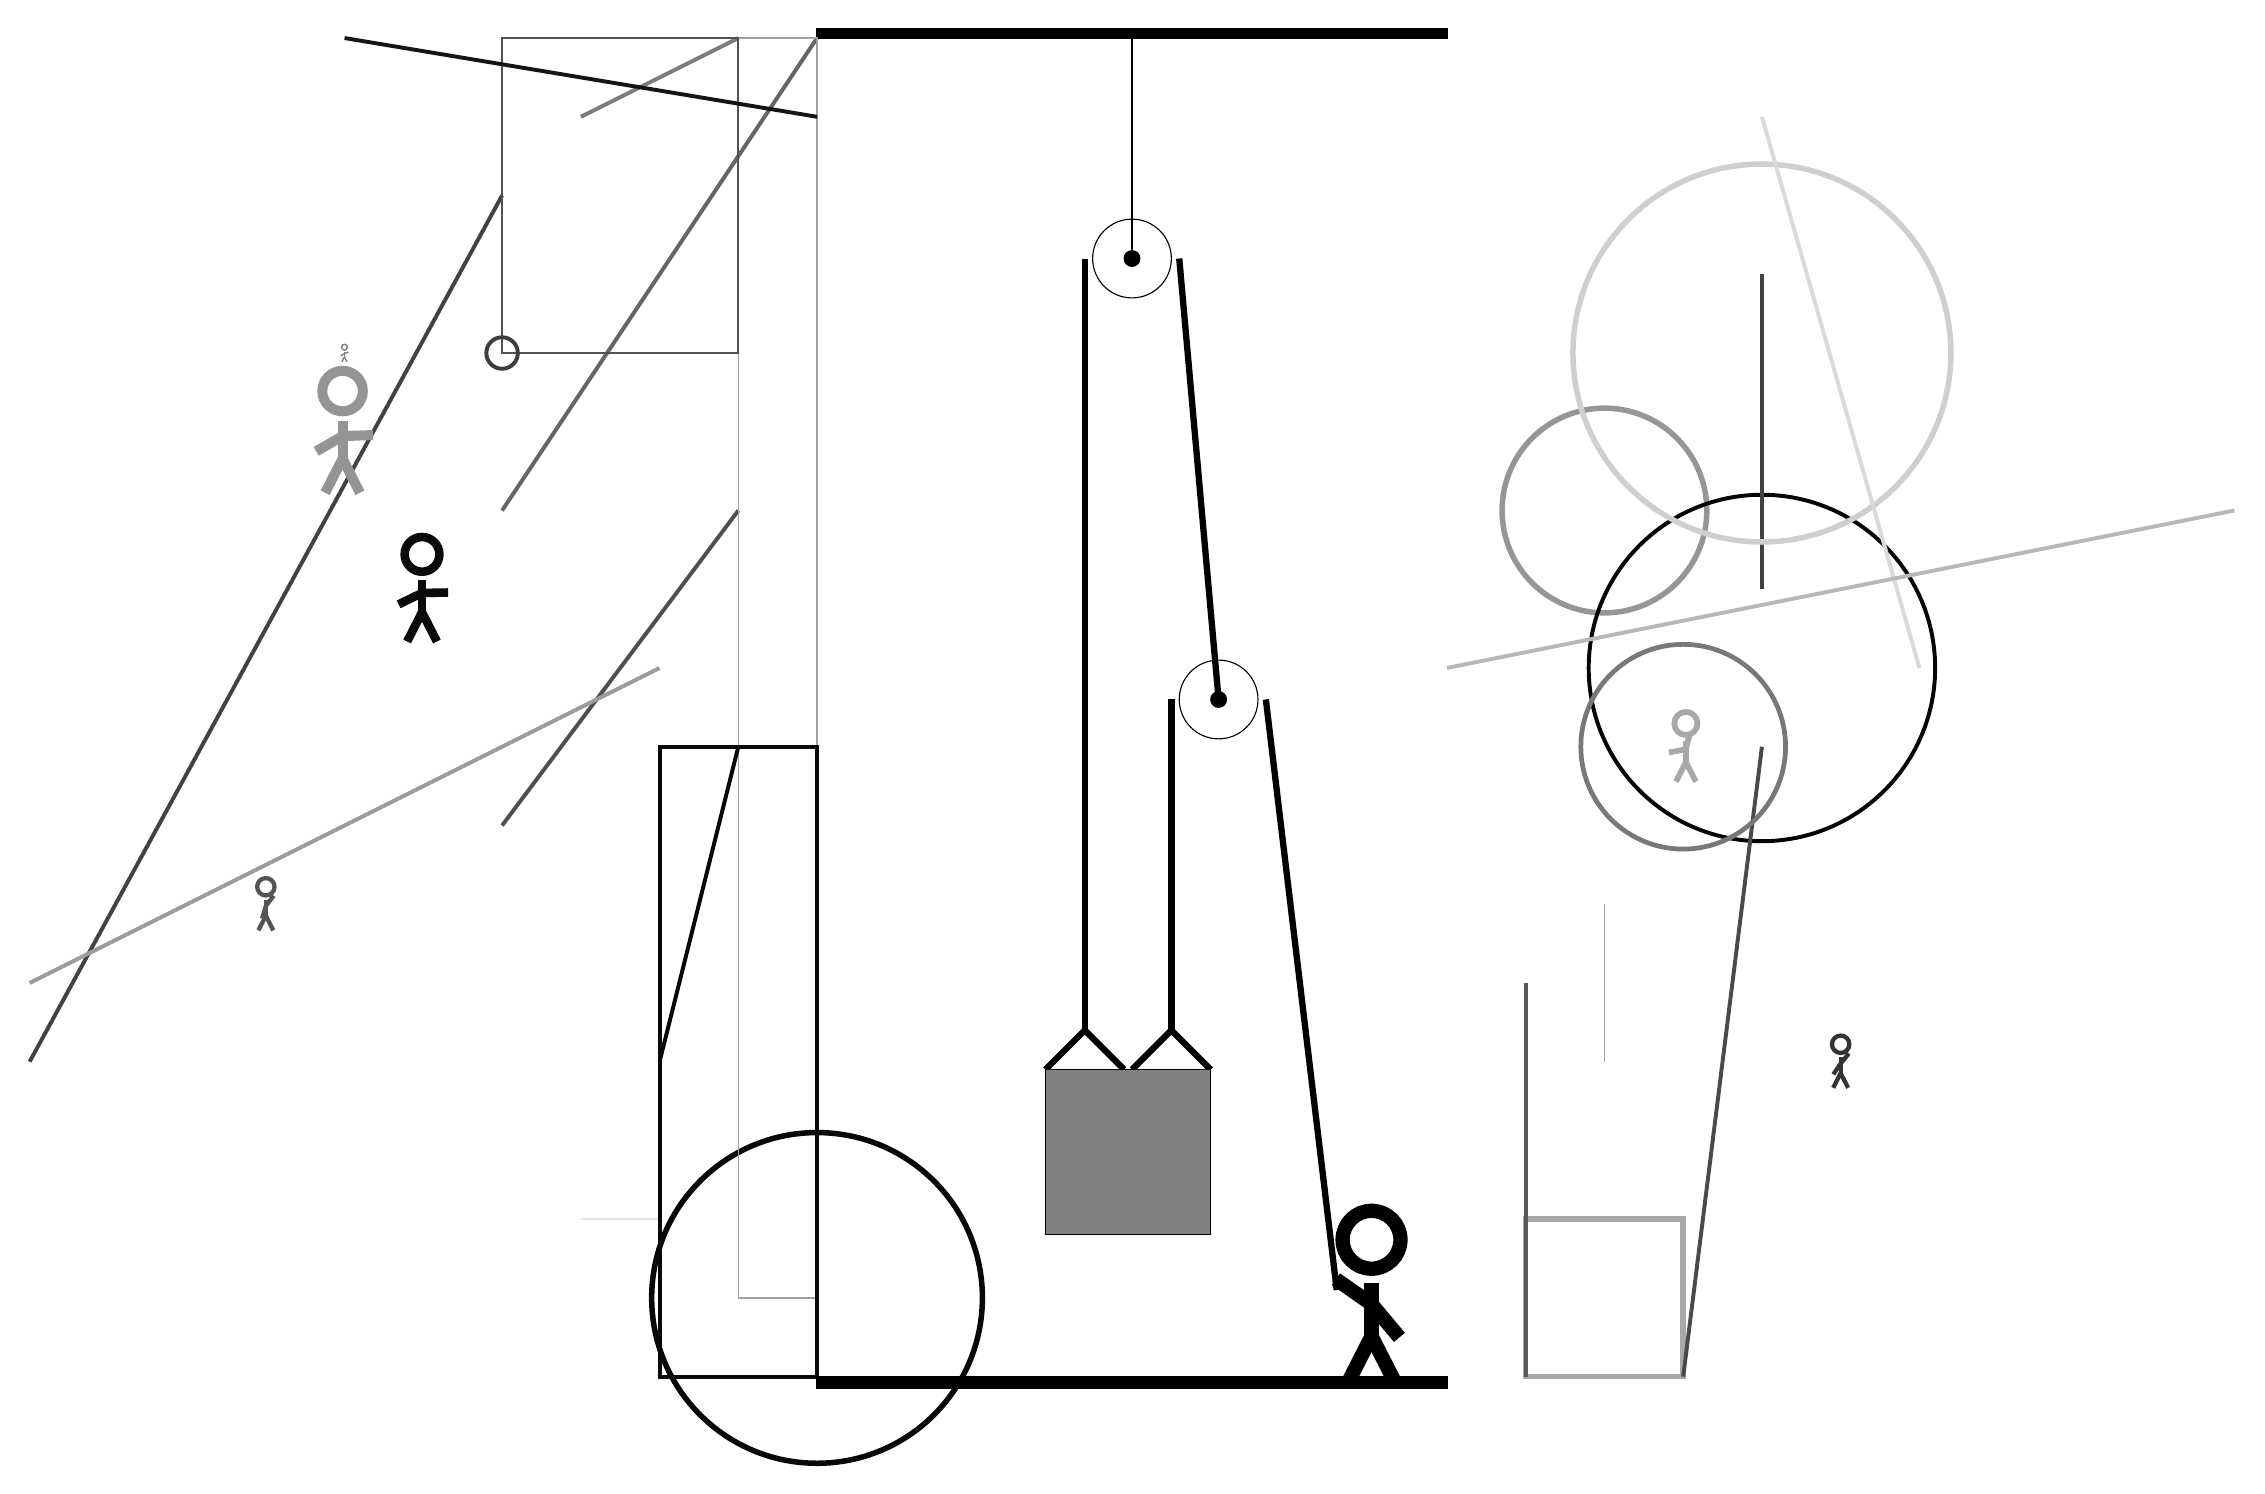
\begin{tikzpicture}
			%%%%% START %%%%%
			
			\draw[fill=black] (-2, 14) rectangle (6, 14.125);
			
			\draw (2, 11.2) circle (0.5);
			\draw[fill=black] (2, 11.2) circle (0.1);
			\draw[thick] (2, 11.2) -- (2, 14);
			
			\draw[line width=0.5mm, color=black!60](-2, 14) -- (-6, 8);
			
			\draw[line width=0.5mm, color=black!51](-3, 14) -- (-5, 13);
			\draw[line width=0.5mm, color=black!74](-6, 12) -- (-12, 1);
			\draw [line width=0.7mm, color=black!41](8, 8) circle (1.3);
			
			\draw [line width=0.5mm, color=black!98](10, 6) circle (2.2);
			
			\draw[line width=0.5mm, color=black!74](10, 11) -- (10, 7);
			
			\node[line width=0.7mm, color=black!80] at (11, 1) {\Strichmaxerl[3][56][51]};
			\draw [line width=0.7mm, color=black!97](-2, -2) circle (2.1);
			\draw [line width=0.7mm, color=black!19](10, 10) circle (2.4);
			\draw[line width=0.5mm, color=black!69](-6, 4) -- (-3, 8);
			\draw[line width=0.7mm, color=black!34] (7, -1) rectangle (9, -3);
			
			\draw[line width=0.2mm, color=black!37] (8, 1) rectangle (8, 3);
			\draw[line width=0.5mm, color=black!71](9, -3) -- (10, 5);
			
			\draw [line width=0.6mm, color=black!53](9, 5) circle (1.3);
			\draw[line width=0.2mm, color=black!10] (-4, -1) rectangle (-5, -1);
			\node[line width=0.2mm, color=black!34] at (9, 5) {\Strichmaxerl[4][11][76]};
			
			\node[line width=0.5mm, color=black!96] at (-7, 7) {\Strichmaxerl[6][26][1]};
			\draw[line width=0.2mm, color=black!37] (-3, 14) rectangle (-2, -2);
			\draw[line width=0.3mm, color=black!68] (-3, 14) rectangle (-6, 10);
			
			\node[line width=0.2mm, color=black!42] at (-8, 9) {\Strichmaxerl[7][30][2]};
			\draw[line width=0.5mm, color=black!39](-4, 6) -- (-12, 2);
			\draw [line width=0.5mm, color=black!76](-6, 10) circle (0.2);
			\draw[line width=0.5mm, color=black!15](10, 13) -- (12, 6);
			\draw[line width=0.5mm, color=black!28](6, 6) -- (16, 8);
			\draw[line width=0.5mm, color=black!65](7, -3) -- (7, 2);
			
			\draw[line width=0.5mm, color=black!96] (-4, -3) rectangle (-2, 5);
			\draw[line width=0.5mm, color=black!97](-4, 1) -- (-3, 5);
			\node[line width=0.7mm, color=black!51] at (-8, 10) {\Strichmaxerl[1][32][22]};
			\draw[line width=0.5mm, color=black!92](-2, 13) -- (-8, 14);
			\node[line width=0.7mm, color=black!67] at (-9, 3) {\Strichmaxerl[3][73][53]};
			
			\draw (3.1, 5.6) circle (0.5);
			\draw[fill=black] (3.1, 5.6) circle (0.1);
			
			\draw[line width = 0.8mm]  (0.9, 0.9) -- (1.4, 1.4) -- (1.9, 0.9);
			\draw[line width = 0.8mm]  (2.0, 0.9) -- (2.5, 1.4) -- (3.0, 0.9);
			\draw[fill=black!50] (0.9, 0.9) rectangle (3.0, -1.2);
			
			\draw[line width = 0.8mm] (1.4, 11.2) -- (1.4, 1.4);
			\centerarc[line width = 0.8mm](2, 11.2)(0:180:0.6);
			\draw[line width = 0.8mm] (2.6, 11.2) -- (3.1, 5.6);
			\draw[line width = 0.8mm] (2.5, 5.6) -- (2.5, 1.4);
			\centerarc[line width = 0.8mm](3.1, 5.6)(0:180:0.6);
			\draw[line width = 0.8mm] (3.7, 5.6) -- (4.6, -1.9);
			
			\node at (5, -2) {\Strichmaxerl[10][-35][-50]};
			
			\draw[fill=black] (-2, -3) rectangle (6, -3.15);
			
			%%%%% END %%%%%
		\end{tikzpicture}
	\end{figure}	
\end{document}